%%
%% Copyright 2007, 2008, 2009 Elsevier Ltd
%%
%% This file is part of the 'Elsarticle Bundle'.
%% ---------------------------------------------
%%
%% It may be distributed under the conditions of the LaTeX Project Public
%% License, either version 1.2 of this license or (at your option) any
%% later version.  The latest version of this license is in
%%    http://www.latex-project.org/lppl.txt
%% and version 1.2 or later is part of all distributions of LaTeX
%% version 1999/12/01 or later.
%%
%% The list of all files belonging to the 'Elsarticle Bundle' is
%% given in the file `manifest.txt'.
%%

%% Template article for Elsevier's document class `elsarticle'
%% with harvard style bibliographic references
%% SP 2008/03/01
%%
%%
%%
%% $Id: elsarticle-template-harv.tex 4 2009-10-24 08:22:58Z rishi $
%%
%%
\documentclass[preprint,authoryear,12pt]{elsarticle}

%% Use the option review to obtain double line spacing
%% \documentclass[authoryear,preprint,review,12pt]{elsarticle}

%% Use the options 1p,twocolumn; 3p; 3p,twocolumn; 5p; or 5p,twocolumn
%% for a journal layout:
%% \documentclass[final,authoryear,1p,times]{elsarticle}
%% \documentclass[final,authoryear,1p,times,twocolumn]{elsarticle}
%% \documentclass[final,authoryear,3p,times]{elsarticle}
%% \documentclass[final,authoryear,3p,times,twocolumn]{elsarticle}
%% \documentclass[final,authoryear,5p,times]{elsarticle}
%% \documentclass[final,authoryear,5p,times,twocolumn]{elsarticle}

%% if you use PostScript figures in your article
%% use the graphics package for simple commands
%% \usepackage{graphics}
%% or use the graphicx package for more complicated commands
%% \usepackage{graphicx}
%% or use the epsfig package if you prefer to use the old commands
%% \usepackage{epsfig}
\usepackage{graphicx}
\usepackage{url}
\usepackage{fullpage}
\usepackage{array}
\graphicspath{{./figures/}}
\DeclareGraphicsExtensions{.pdf,.png,.jpg}

%% The amssymb package provides various useful mathematical symbols
\usepackage{amssymb}
\usepackage{amsmath}
%% The amsthm package provides extended theorem environments
%% \usepackage{amsthm}

%% The lineno packages adds line numbers. Start line numbering with
%% \begin{linenumbers}, end it with \end{linenumbers}. Or switch it on
%% for the whole article with \linenumbers after \end{frontmatter}.
%% \usepackage{lineno}

%% natbib.sty is loaded by default. However, natbib options can be
%% provided with \biboptions{...} command. Following options are
%% valid:

%%   round  -  round parentheses are used (default)
%%   square -  square brackets are used   [option]
%%   curly  -  curly braces are used      {option}
%%   angle  -  angle brackets are used    <option>
%%   semicolon  -  multiple citations separated by semi-colon (default)
%%   colon  - same as semicolon, an earlier confusion
%%   comma  -  separated by comma
%%   authoryear - selects author-year citations (default)
%%   numbers-  selects numerical citations
%%   super  -  numerical citations as superscripts
%%   sort   -  sorts multiple citations according to order in ref. list
%%   sort&compress   -  like sort, but also compresses numerical citations
%%   compress - compresses without sorting
%%   longnamesfirst  -  makes first citation full author list
%%
%% \biboptions{longnamesfirst,comma}

% \biboptions{}

\journal{International Journal of Forecasting}

\begin{document}

\begin{frontmatter}

%% Title, authors and addresses

%% use the tnoteref command within \title for footnotes;
%% use the tnotetext command for the associated footnote;
%% use the fnref command within \author or \address for footnotes;
%% use the fntext command for the associated footnote;
%% use the corref command within \author for corresponding author footnotes;
%% use the cortext command for the associated footnote;
%% use the ead command for the email address,
%% and the form \ead[url] for the home page:
%%
%% \Title{Title\tnoteref{label1}}
%% \tnotetext[label1]{}
%% \author{Name\corref{cor1}\fnref{label2}}
%% \ead{email address}
%% \ead[url]{home page}
%% \fntext[label2]{}
%% \cortext[cor1]{}
%% \address{Address\fnref{label3}}
%% \fntext[label3]{}

\title{Forecasting Elections with Non-Representative Polls\footnote{We
    thank the National Science Foundation for partial support of this research.}}

%% use optional labels to link authors explicitly to addresses:
%% \author[label1,label2]{<author name>}
%% \address[label1]{<address>}
%% \address[label2]{<address>}


\author[col]{Wei Wang}
\ead{ww2243@columbia.edu}


\author[msr]{David Rothschild}
\ead{davidmr@microsoft.com}


\author[msr]{Sharad Goel}
\ead{sharadg@microsoft.com}


\author[col,poly]{Andrew Gelman}
\ead{gelman@stat.columbia.edu}

\address[col]{Department of Statistics, Columbia University, New York, NY, USA}
\address[msr]{Microsoft Research, New York, NY, USA}
\address[poly]{Department of Political Science, Columbia University, New York, NY, USA}

\begin{abstract}
%% Text of abstract
  Election forecasts have traditionally been based on representative polls,
  in which randomly sampled individuals are asked for whom they intend to vote.
  % Ever since the debacle of the \textsl{Literary Digest} poll in the 1936
  % election,
  % representative polling has been considered the standard in election
  % forecasting, via the ubiquitous voter intention poll.
  While representative polling has historically proven to be quite effective, it
  comes at considerable financial and time costs. Moreover, as response rates have declined
  over the past several decades, the statistical benefits of representative
  sampling have diminished.
  %as the costs have increased even further.
  In this paper, we show that with proper statistical
  adjustment, non-representative polls can be used to generate accurate election
  forecasts, and often faster and at less expense than traditional survey
  methods.  We demonstrate this approach by creating forecasts from a novel and
  highly non-representative survey dataset: a series of daily voter intention
  polls for the 2012 presidential election conducted on the Xbox gaming platform.
  After adjusting the Xbox responses via multilevel regression and
  poststratification, we obtain estimates in line with forecasts from leading
  poll analysts, which were based on aggregating hundreds of traditional polls
  conducted during the election cycle. We conclude by arguing that
  non-representative polling shows promise not only for election forecasting, but
  also for measuring public opinion on a broad range of social, economic and
  cultural issues.
\end{abstract}

\begin{keyword}
%% keywords here, in the form: keyword \sep keyword

%% MSC codes here, in the form: \MSC code \sep code
%% or \MSC[2008] code \sep code (2000 is the default)
  Non-representative polling \sep multilevel regression and poststratification
  \sep election forecasting
\end{keyword}

\end{frontmatter}

%%
%% Start line numbering here if you want
%%
% \linenumbers

%% main text
\section{Introduction}
At the heart of modern opinion polling is representative sampling, built around
the goal that every individual in a particular target population (e.g., registered or likely U.S. voters)
has the same probability of being sampled. From address-based,
in-home interview sampling in the 1930s to random digit dialing after the growth
of landlines and cellphones, leading polling organizations have put immense
effort into obtaining %random draws of
representative samples.

The wide-scale adoption of representative polling can largely be traced to a
pivotal polling mishap in the 1936 U.S. presidential election campaign.  During
that campaign, the popular magazine \textsl{Literary Digest} conducted a mail-in
survey that attracted over two million responses, a huge sample even by modern standards.
The magazine, however, incorrectly predicted a landslide victory for
Republican candidate Alf Landon over the incumbent Franklin Roosevelt.  Roosevelt,
in fact, decisively won the election, carrying every state except for Maine and
Vermont.  As pollsters and academics have since pointed out, the magazine's pool
of respondents was highly biased: it consisted mostly of auto and telephone
owners as well as the magazine's own subscribers, which underrepresented
Roosevelt's core constituencies \citep{squire19881936}.  During that same
campaign, pioneering pollsters, including George Gallup, Archibald Crossley, and
Elmo Roper, used considerably smaller but representative samples to predict the
election outcome with reasonable accuracy \citep{gosnell1937technical}.
%This is widely viewed as the single event that sealed
%the supremacy of representative polling.
Accordingly, non-representative or ``convenience sampling'' rapidly
fell out of favor with polling experts.

So why do we revisit this seemingly long-settled case? Two recent trends
spur our investigation.
First, representative sampling is not nearly as representative as its name
suggests, and it is becoming less so. Random digit dialing (RDD), the standard
method in modern representative polling, has suffered increasingly high
non-response rates, both
due to the general public's growing reluctance to answer phone surveys,
%respond (a quite reasonable reluctance given the massive volume of
%telephone polling that is now being done, especially in battleground states during election years)
and expanding technical means to screen unsolicited calls
\citep{keeter2006gauging}. By one measure, RDD response rates have decreased from 36\% in 1997 to 9\% in 2012
\citep{kohut2012assessing}. With such low response rates, even if the initial pool of targets is representative,
those who ultimately answer the phone and elect to respond are almost certainly not, calling into question the statistical benefits of such an approach.
% the representativeness of the polls conducted using standard survey
%methodology is an increasing concern.
%While standard polls have preformed well in recent cycles, there is a meaningful possibility that
%the response rates could cause a major problem in the near future.
Related to dropping response rates is a corresponding increase in cost, in both time and money, as one needs to contact more and more potential respondents to find one willing to participate.
The second trend driving our research is that with recent technological innovations, it is increasingly convenient and cost-effective to collect large numbers of highly non-representative samples via online surveys.
What took several months for the
\textsl{Literary Digest} editors to collect in 1936 can now take only a
few days and can cost just pennies per response.
%How to
%draw useful conclusions from this big data has become an interesting and
%important issue facing researchers and pollsters.
The challenge, of course, is to extract meaningful signal from these unconventional samples.

In this paper, we show that with proper statistical adjustment,
non-representative polls yield accurate presidential election forecasts, on par with
those based on traditional representative polls.
We proceed as follows. Section 2 describes the
election survey that we conducted on the Xbox gaming platform during the 45 days leading up to the
2012 U.S. presidential race.
%election and shows its raw response and demographic breakdown.
Our Xbox sample is
highly biased in two key demographic dimensions, gender and age, and the raw
responses accordingly disagree with the actual outcomes. The statistical
techniques we use to adjust the raw estimates are introduced in two stages.
In Section 3, we construct daily estimates of
voter intent via multilevel regression and poststratification (MRP).
The central idea of MRP is to partition the data into thousands of
demographic cells, estimate voter intent at the cell level with a multilevel regression model, and finally
to aggregate cell-level estimates in accordance with the target population's demographic composition.
Estimates of daily voter intent, however, do not immediately translate to
election day forecasts. For example, there is a known anti-incumbency bias in voter intention polls.
Section 4 describes how to transform voter intent to
projections of vote share and electoral votes.
%We also discuss assumptions and robustness of our method in Section 4,
%while Section 5 compares
%our results with predictions based on other approaches.
We conclude in Section 5 by discussing the potential for non-representative polling in other domains.

\section{Xbox data}
Our analysis is based on an opt-in poll continuously available on the Xbox
gaming platform during the 45 days preceding the 2012 U.S. presidential
election.  Each day, three to five questions were posted, one of which gauged
voter intention with the standard query, ``If the election were held today, who
would you vote for?".  Respondents were allowed to answer at most once per
day. The first time they participated in an Xbox poll, respondents were
additionally asked to provide basic demographic information about themselves,
including their sex, race, age, education, state, party ID, political ideology,
and for whom they voted in the 2008 presidential election. In total, 750,148
interviews were conducted with 345,858 unique respondents---over 30,000 of whom
completed five or more polls---making this one of the largest ever election
panel studies.
%who each time indicated the candidate for whom they intended to
%vote, and over 30,000 unique respondents completed 5 or more polls,
%Attracting over 16,000 respondents per day, our Xbox poll is in fact larger than all of the standard polling combined.
%The respondents also provided demographic information about themselves prior to the first time they responded.

%This novel dataset provides a unique opportunity for academics and pollsters to
%understand the voting behaviors of Americans exhibited in the 2012 presidential
%election. However, how to utilize of the rich information contained in the data
%set also presents us challenges.

\begin{figure}
  \centering
  \includegraphics[width=\textwidth]{"xbox_electorate_demo_comp"}
  \caption{A comparison of the demographic, partisan, and 2008 vote
    distribution in the Xbox dataset and the 2012 electorate (as
    measured by adjusted exit polls). The sex and age distributions, as one might expect, exhibit
  considerable differences.}
  \label{fig:demo_comp}
\end{figure}

\begin{figure}
  \centering
  \includegraphics[width=.8\textwidth]{"raw_response"}
  \caption{Daily (unadjusted) Xbox estimates of two-party Obama support during
    the 45 days leading up to the 2012 presidential election, which suggest a
    landslide victory for Mitt Romney. The dotted blue line indicates a
    consensus average of traditional polls (the daily aggregated polling results from Pollster.com), the horizontal dashed line at 52\%
    indicates the actual two-party vote share obtained by Barack Obama, and the
    vertical dotted lines give the dates of the three presidential debates.}
  \label{fig:raw_responses}
\end{figure}

Despite the large sample size, the pool of Xbox respondents is far from representative of the voting population.
Figure~\ref{fig:demo_comp} compares the demographic composition of the Xbox participants to that of the general electorate, as estimated via
the 2012 national exit poll.\footnote{For ease of interpretation, in Figure~\ref{fig:demo_comp} we group states into 4 categories: (1) battleground states
(Colorado, Florida, Iowa, New Hampshire, Ohio, and Virginia), the five
states with the highest amounts of TV spending plus New Hampshire, which had the highest per-capita spending; (2) quasi-battleground
  states (Michigan, Minnesota, North Carolina, Nevada, New Mexico, Pennsylvania,
  and Wisconsin), which round out the states where the campaigns and their affiliates made major TV buys; (3) solid Obama states (California, Connecticut, District
  of Columbia, Delaware, Hawaii, Illinois, Maine, Maryland, Massachusetts, New
  Jersey, New York, Oregon, Rhode Island, Vermont, and Washington); and (4) solid Romney
  states (Alabama, Alaska, Arizona, Arkansas, Georgia, Idaho, Indiana,
  Kansas, Kentucky, Louisiana, Mississippi, Missouri, Montana, Nebraska, North
  Dakota, Oklahoma, South Carolina, South Dakota, Tennessee, Texas, Utah, West
  Virginia, and Wyoming).}
 %shows the comparison between the Xbox survey
%respondents and 2012 national exit poll respondents (which, though not exact, is
%taken as the proxy of the ground truth) in terms of several key demographic and
%partisan variables, including sex, race, age, education, contestedness of state, party identification, ideology as well as 2008 vote.\footnote{We did not use 2012 national exit poll to get the breakdown of the 2008
 % vote of the respondents, because it was not asked, so we used the actual vote breakdown instead.}
The most
striking differences are for age and sex. As one might expect, young men dominate the Xbox population: 18-to-29-year-olds
comprise 65\% of the Xbox dataset, compared to 19\% in the exit poll; and men make up
93\% of the Xbox sample but only 47\% of the electorate.  Political
scientists have long observed that both age and sex are strongly correlated with
voting preferences \citep{kaufmann1999changing}, and indeed these discrepancies are apparent in the unadjusted
time-series of Xbox voter intent shown in Figure \ref{fig:raw_responses}.
%These differences must go a long way in explaining the awry raw
%results.
In contrast to estimates based on traditional, representative polls (indicated by the dotted blue line in Figure \ref{fig:raw_responses}),
the uncorrected Xbox sample suggests a landslide victory for Mitt Romney, reminiscent of the
infamous \textsl{Literary Digest} error.
%Romney landslide in the 2012 election. This is reminiscent of the poor results obtained from the
%\textsl{Literary Digest} survey, which also made no attempt to be representative of the general population.

% For other variables, the differences seem much less stark. Particularly, the
% differences in party identification, ideology and 2008 vote breakdown seem
% surprising small, which might be explained by that the effects of the influx of
% young people (who tend to be more liberal) and the influx of males (who tend to
% be more conservative) in the Xbox data cancel out each other.


\section{Estimating voter intent with multilevel regression and poststratification}
\label{sec:mrp}
\subsection{Multilevel regression and poststratification}
To transform the raw Xbox data into accurate estimates of voter intent in the general electorate, we
make use of the rich demographic information that respondents provide.
In particular we \emph{poststratify} the raw Xbox responses to mimic a representative sample of likely voters.
Poststratification is a popular method for correcting for known differences
between sample and target populations \citep{little1993post}.
%We use notation $X$
%for the known variables in the population (we assume that they are categorical),
%and $y$ for the outcome of interest.
The core idea is to partition the population into cells (e.g., based on combinations of various demographic attributes), use the sample to estimate the response variable within each
cell, and finally to aggregate the cell-level estimates up to a population-level estimate by weighting each cell by its relative proportion in the population.
%The poststratification cells $j$, which are
%defined by combinations of $X$, have population sizes $N_j$. The poststratified
Using $y$ to indicate the outcome of interest, the poststratification estimate is defined by,
%estimate of $y$ at the population level is given by
\[\hat{y}^{\text{PS}}=\frac{\sum_{j=1}^JN_j\hat{y}_j}{\sum_{j=1}^JN_j}\]
where $\hat{y}_j$ is the estimate of $y$ in cell $j$, and $N_j$ is the size of the $j$-th cell in the population.
We can analogously
derive an estimate of $y$ at any subpopulation level $s$ (e.g., voter intent in a particular state)
by
\[\hat{y}_s^{\text{PS}}=\frac{\sum_{j\in J_s}N_j\hat{y}_j}{\sum_{j\in J_s}N_j}\]
where $J_s$ is the set of all cells that comprise $s$. As is readily apparent from the form of the poststratification estimator, the key is to obtain accurate cell-level estimates,
as well as estimates for the cell sizes.

One of the most common ways to generate cell-level estimates is to simply average sample responses within each cell.
If we assume that within a cell the sample is drawn at random from the larger population, this yields an unbiased estimate.
%The underlying assumption of poststratification is that simple random sampling
%holds within each of the $J$ poststrata.
However, this assumption of cell-level simple random sampling is only reasonable when
the partition is sufficiently fine; on the other hand, as the partition becomes finer,
the cells become sparse, and the empirical sample averages become unstable.
We address these issues by instead generating cell-level estimates via a regularized regression model, namely
multilevel regression.
% to
%improve the estimates $y_s$, which we use later for constructing the estimates at
%the aggregated levels.
This combined model-based poststratification strategy,
known as multilevel regression and poststratification (MRP), has been used to
obtain accurate small-area subgroup estimates, such as for public opinion and voter turnout in individual states and demographic subgroups \citep{park2004bayesian, lax_2009, ghitza_2013}.

More formally, applying MRP in our setting comprises two steps. First a Bayesian hierarchical model is fit to obtain estimates for sparse
poststratification cells; second, one averages over the cells, weighting by a measure of forecasted voter turnout, to get state and national-level estimates. Specifically, we generate the cells by considering all possible combinations of sex (2 categories), race (4 categories), age (4 categories), education
(4 categories), state (51 categories), party ID (3 categories), ideology (3
categories) and 2008 vote (3 categories), which partition the data into 176,256
cells.\footnote{All demographic variables are collected prior to respondents' first poll, alleviating concerns that respondents may adjust their demographic responses to be inline with their voter intention (e.g., a new Obama supporter switching his or her party ID from Republican to Democrat).} We fit two, nested multilevel logistic regressions to estimate
candidate support in each cell. The first of the two models predicts
whether a respondent supports a major-party candidate (i.e., Obama or Romney), and the
second predicts support for Obama given that the respondent supports a
major-party candidate. Following the notation of \citet{gelman2007data}, the
first model is given by
\begin{align}\label{eqn:m1}
  \text{Pr}(Y_i \in \, &\{\text{Obama, Romney}\})=\nonumber\\
  &\text{logit}^{-1}\big(\alpha_0+  \alpha_1\text{(state last vote share)} \\
  &+ a^{\text{state}}_{j[i]}+a^{\text{edu}}_{j[i]}+a^{\text{sex}}_{j[i]}+a^{\text{age}}_{j[i]}
  +a^{\text{race}}_{j[i]}+a^{\text{party ID}}_{j[i]}
  +b^{\text{ideology}}_{j[i]} + b^{\text{last vote}}_{j[i]} \big)\nonumber
\end{align}
where $\alpha_0$ is the fixed baseline intercept, and
$\alpha_1$ is the fixed slope for Obama's fraction of two-party
vote share in the respondent's state in the last presidential election.
The terms $a^{\text{state}}_{j[i]}$, $a^{\text{edu}}_{j[i]}$, $a^{\text{sex}}_{j[i]}$ and so on---which in general we denote by $a^{\text{var}}_{j[i]}$---correspond to varying coefficients associated with each categorical variable.
%, and var represents any categorical predictor
%included in the model.
Here the subscript $j[i]$ indicates the cell to which the $i$-th
respondent belongs. For example, $a^{\text{age}}_{j[i]}$ takes values
from $\{a^{\text{age}}_{18-29}, a^{\text{age}}_{30-44}, a^{\text{age}}_{45-64},
a^{\text{age}}_{65+}\}$ depending on the cell membership of the $i$-th
respondent. The varying coefficients $a_{j[i]}^{\text{var}}$ are given independent prior
distributions \[a^{\text{var}}_{j[i]}\sim N(0,\sigma^2_\text{var}).\] To complete the
full Bayesian specification, the variance parameters are assigned a hyperprior
distribution \[\sigma^2_\text{var}\sim \text{inv-}\chi^2(\nu, \sigma_0^2),\] with a
weak prior specification for the remaining parameters, $\nu$ and $\sigma_0$.
%%  \text{var}=\text{sex}, \text{race}, \text{age}, &\text{edu}, \text{state},
%%  \text{party ID}, \text{ideology}, \text{2008 vote}
The benefit of using a multilevel model is that estimates for
relatively sparse cells can be improved through ``borrowing strength'' from
demographically similar cells that have richer data. Similarly, the second model
is defined by
\begin{align}  \label{eqn:m2}
  \text{Pr}(Y_i = \, &\text{Obama} \, |\, Y_i\in\{\text{Obama, Romney}\})=\nonumber\\
  &\text{logit}^{-1}\big(\beta_0+ \beta_1\text{(state last vote share)} \\
  & + b^{\text{state}}_{j[i]}+b^{\text{edu}}_{j[i]}+b^{\text{sex}}_{j[i]}+b^{\text{age}}_{j[i]}
  +b^{\text{race}}_{j[i]}+b^{\text{party ID}}_{j[i]} +
  b^{\text{ideology}}_{j[i]} + b^{\text{last vote}}_{j[i]}
 \big)\nonumber
\end{align}
and
\begin{align*}
  b^{\text{var}}_{j[i]}&\sim N(0,\eta^2_\text{var}),\\
  \eta^2_\text{var}&\sim \text{inv-}\chi^2(\mu, \eta_0^2).
%%  \text{var}=\text{sex}, \text{race}, \text{age}, &\text{edu}, \text{state},
%%  \text{party ID}, \text{ideology}, \text{2008 vote}
\end{align*}
Jointly, Eqs.\ \eqref{eqn:m1} and \eqref{eqn:m2} define a Bayesian model
that describes the data. Ideally, we would perform a fully Bayesian
analysis to obtain the posterior distribution of the parameters. However, for
computational convenience, we use the approximate marginal maximum likelihood
estimates obtained from the \texttt{glmer()} function in the \texttt{R} package
\texttt{lme4} \citep{bates2013lme4}.

Having detailed the multilevel regression step, we now turn to poststratification, where cell-level estimates are weighted by the proportion
of the electorate in each cell and aggregated to the appropriate level (e.g., state or national).
%that we are
%interested in. For example, state level two-party Obama support can be calculated
%by
%\[\theta_S=\frac{\sum_{j\in J_S}N_j\theta_j}{\sum_{j\in J_S}N_j}\]
%where $\theta_j$ is the two-party Obama support in cell $j$, $N_j$ is the
%population size of the cell $j$ and $J_S$ is the set of all cells that comprise
%state $S$.
To compute cell weights, we require cross-tabulated population data.  One
commonly used source for such data is the Current Population Survey (CPS);
however, the CPS does not includes some key poststratification
variables, such as party identification.  We thus
instead use exit poll data from the 2008 presidential election. Exit polls
are conducted on election day outside voting stations to record the choices of
exiting voters, and they are generally used by researchers and news media to
analyze the demographic breakdown of the vote (after a post-election
adjustment that aligns the weighted responses to the reported
state-by-state election results). In total, 101,638 respondents were
surveyed in the state and national exit polls.
%Exit polling data are
%available at the both national and state levels; we use the national exit poll results as
%to
%our poststratification population when the outcome is the national vote share,
%and state exit polls when the outcomes are the state vote shares.
We use the exit poll from 2008, not 2012, because this means that in
theory our method as described here could have been used to generate
real-time predictions during the 2012 election campaign.
Admittedly, this approach puts our
prediction at a disadvantage since we cannot capture the demographic shifts of the intervening four years.
%, that is, we are essentially
%generating daily voter intents for the 2008 electorate.
While combining exit poll and CPS data would arguably yield improved results, for simplicity and
transparency we exclusively use the 2008 exit poll summaries for our poststratification.

\subsection{National and state voter intent}
Figure~\ref{fig:national_snap} shows the adjusted
two-party Obama support for the last 45 days of the election.
%The daily voter intents for two-party Obama support at the national level are
%illustrated in Figure \ref{fig:national_snap}.
Compared with the uncorrected estimates in
Figure \ref{fig:raw_responses}, the MRP-adjusted estimates yield a much
more reasonable timeline of Obama's standing over the course of the final weeks of the
campaign.
With a clear advantage at the beginning, Obama's support
slipped rapidly after the first presidential debate---though never falling below
50\%---and gradually recovered, building up a decisive lead in the final days.

On the day before the election, our estimate of voter intent  is off by a mere 0.6
percentage points from the actual outcome (indicated by the dotted horizontal
line).  Voter intent in the weeks prior to the election does not directly equate
to an estimate of vote share on election day---a point we return to in
Section~\ref{sec:forecast}. As such, it is difficult to evaluate the accuracy of
our full time-series of estimates.  Nonetheless, we note that our estimates are
not only intuitively reasonable, but that they are also inline with prevailing
estimates based on traditional, representative polls. In particular, our
estimates roughly track---and are even arguably better than---those from Pollster.com, one of the leading poll aggregators during the 2012
campaign.

%While it is hard to evaluate the accuracy of our estimates in the weeks prior to the election (since
%But we should not interpret these voter
%intents based on 2008 exit polls as the forecasts for the 2012 electorate
%votes. The confidence bands of the MRP adjusted voter intent represent the
%uncertainty about our estimates voter intents if the 2012 electorate are the same
%as the respondents in the 2008 exit poll.

\begin{figure}
  \centering
  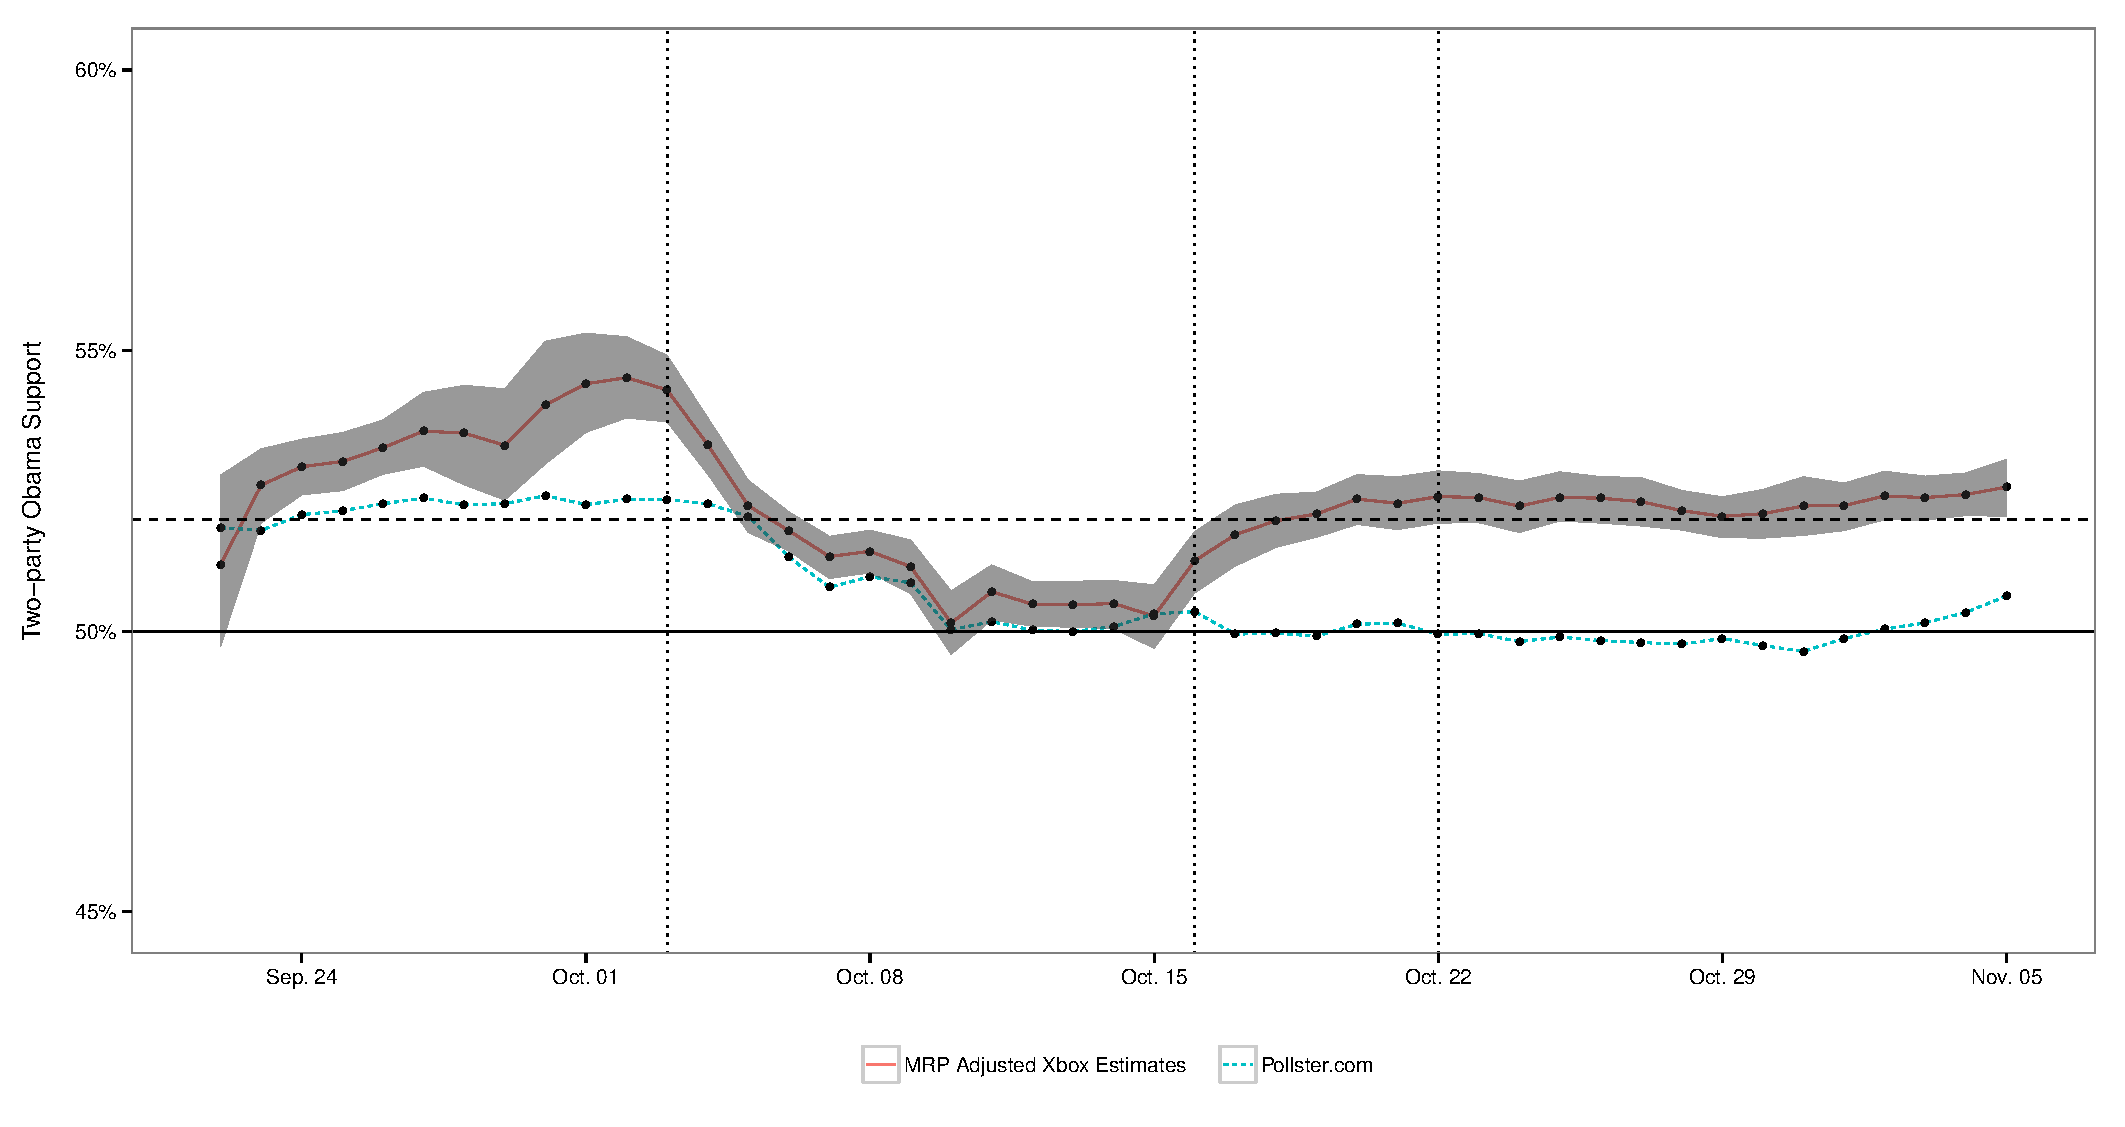
\includegraphics[width=.8\textwidth]{mrp_snapshots_national}
  \caption{National MRP-adjusted voter intent of two-party Obama support over
    the 45-day period and the associated 95\% confidence bands. The horizontal
    dashed line indicates the actual two-party Obama vote share. The three
    vertical dotted lines indicate the presidential debates. Compared with the raw
    responses in Figure \ref{fig:raw_responses}, the MRP-adjusted voter intent
    is much more reasonable, and voter intent in the last few days is very
    close to the actual outcome. For comparison, the daily aggregated polling
    results from Pollster.com, shown as the blue dotted line, are further away from the actual vote share
    than the estimates generated from the Xbox data in the last few days.}
  \label{fig:national_snap}
\end{figure}

National vote share receives considerable media attention, but
state-level estimates are particularly relevant for many stakeholders given the role of the Electoral College in selecting the winner \citep{rothschild2013combining}.
%For forecasting the winner of the Electoral College, the relevant result for most stakeholder, one needs to forecast the joint probability of victory for each candidate in
%the 51 Electoral College races
Forecasting state-by-state
races is a challenging problem due to the
interdependencies in state outcomes,
%and the joint electoral votes has not yet become the standard forecast
the logistical difficulties of measuring state-level vote preference,
%lack
%of complete state specific poll tracking,
and the effort required to combine information from various sources \citep{lock_2010}.
%[2010] Bayesian combination of state polls and election forecasts. {\em Political Analysis} {\bf 18}, 337--348. (Kari Lock and Andrew Gelman)
The MRP framework, however, provides a straightforward methodology for generating state-level results.
Namely, we use the same cell-level estimates employed in the national estimate,
as generated via the multilevel model in Eqs.\ \eqref{eqn:m1} and
\eqref{eqn:m2}, and we then poststratify to each state's demographic composition.
%2008 state exit polls, w
%e can construct
In this manner, the Xbox responses can be used to construct
estimates of voter intent over the last 45 days of the campaign for all 51 Electoral College races.

%daily MRP adjusted voter intents of two-party Obama support over the 45-day
%periods for all 51 Electoral College races.
Figure \ref{fig:state_snap} shows two-party Obama support for the 12 states with the most electoral votes.
%The
%comment on interpretation of the confidence bands in the national daily voter
%intents applies here too.
The state timelines share similar trends (e.g., support for Obama dropping after
the first debate), but also have their own idiosyncratic movements, an indication
of a reasonable blend of national and state-level signals.
%For 48 of the 51 races, the
%MRP-adjusted estimates in the last few days before the election correctly
%indicate whether the state went Democrat or Republican.  The two exceptions are
%Florida and North Carolina, which we missed by about one percentage point, and
%which were the two states with the smallest margins of victory across the 51 races.
To demonstrate the accuracy of the MRP-adjusted estimates, we plot, in
dotted blue lines in Figure~\ref{fig:state_snap}, the estimates generated by
Pollster.com, which are broadly consistent with our state-level MRP estimates.
Moreover, across the 51 Electoral College races, the mean and median absolute errors of 
our estimates on the day before the election 
are just 2.5 and 1.8 percentage points, respectively.

\begin{figure}
  \centering
  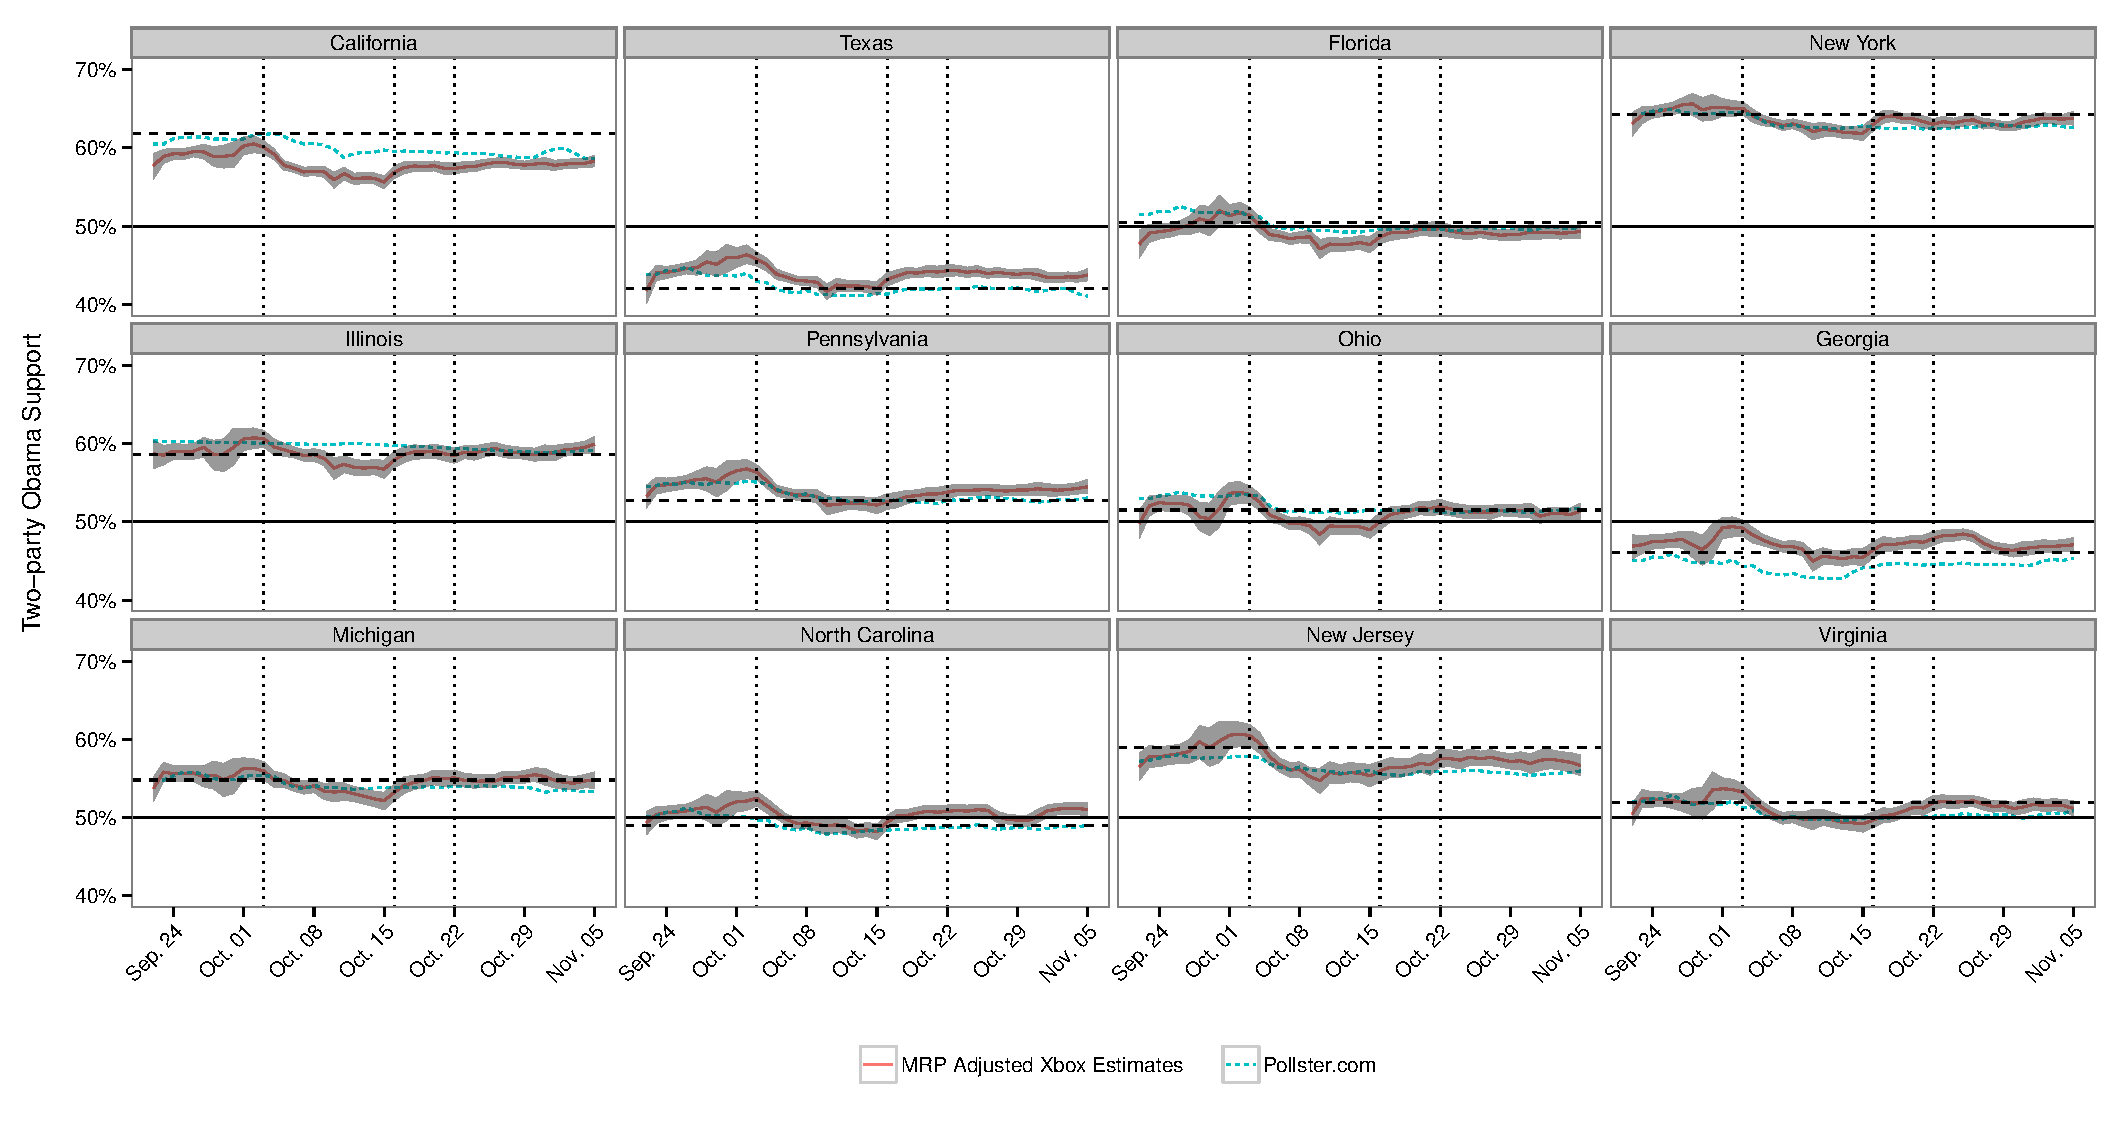
\includegraphics[width=15cm]{mrp_snapshots_state}
  \caption{MRP-adjusted daily voter intent for the 12 states with the most electoral
    votes, and the associated 95\% confidence bands. The horizontal dashed lines
    in each panel give the actual two-party Obama vote shares in that
    state. The mean and median absolute errors of the last day voter intent
    across the 51 Electoral College races are 2.5 and 1.8 percentage points,
    respectively. The state-by-state daily aggregated polling results from
    Pollster.com, given in the dotted blue lines, are broadly consistent with
    the estimates from the Xbox data.}
  \label{fig:state_snap}
\end{figure}


\subsection{Voter intent for demographic subgroups}
Apart from Electoral College races, election
forecasting often focuses on candidate preference among demographic
subpopulations. Such forecasts are of significant importance in modern political
campaigns, which often employ targeted campaign strategies \citep{hillygus2009persuadable}. In the
highly non-representative Xbox survey, certain
subpopulations are heavily underrepresented and plausibly suffer from
strong self-selection problems. This begs the question, can we reasonably expect to estimate
the views of older women on a platform that largely caters to young men?

\begin{figure}
  \centering
  \includegraphics[width=\textwidth]{"demo_group_marginals"}
  \caption{Comparison of two-party Obama vote share for various demographic subgroups,
  	as estimated from the 2012 national exit poll and from the Xbox data on the day before the election.
    %voter intent and 2012 national exit poll in marginal subgroups defined by sex,
    %race, age, education, contestedness of state, party identification, ideology
    %and 2008 vote. The ``how did you vote in the previous election'' question was not asked in the 2012
    %national exit poll questionnaire, so only Xbox results are available for the
    %last panel.
    }
  \label{fig:marginal_comp}
\end{figure}

\begin{figure}
  \centering
  \includegraphics[width=.6\textwidth]{"demo_groups_two_way_interaction"}
  \caption{Two-party Obama support as estimated from
  the 2012 national exit poll and from the Xbox data on the day before the election,
%   support based on the last day MRP
    %voter intent and 2012 national exit poll
    for various two-way interaction demographic subgroups (e.g., 65+ year-old women).
    %defined by variables including sex, race, age, education, party
    %identification and ideology.
    The sizes of the dots are proportional to the
    population sizes of the corresponding subgroups. Subgroups within the same
    two-way interaction category (e.g., age by sex) have the same color.}
  \label{fig:two_way_comp}
\end{figure}

It is straightforward in MRP to estimate
voter intent among any collection of demographic cells: we again use the same cell-level estimates as in the
national and state settings, but poststratify to the desired target population. For example, to estimate
voter intent among women, the poststratification weights are based on the relative number of women in each demographic cell.
%MRP adjusted voter intents can be generated using the same cell-level estimates
%and the same poststratification population (the 2008 national exit poll), but
%aggregating to levels other than state (e.g., age, education or
%race-by-education).
To illustrate this approach, we compute Xbox estimates of Obama support for each
level of our categorical variables (e.g., males, females, Whites, Blacks, etc.)
on the day before the election, and compare those with the actual voting
behavior of those same groups as estimated by the 2012 national exit poll.  As
seen in Figure~\ref{fig:marginal_comp}, the Xbox estimates are remarkably
accurate, with a median absolute difference of 1.5 percentage points between
the Xbox and the exit poll numbers.\footnote{Respondents' 2008 vote was not asked on
  the 2012 exit poll, so we exclude that comparison from
  Figure~\ref{fig:marginal_comp}.}
%comparisons across marginal subgroups, and we can see that MRP estimates are very
%precise at this level.
%based on the last day MRP
%adjusted voter intent with the reference two-party Obama vote shares calculated
%from the 2012 national exit poll, at the marginal levels and two-way interaction
%levels defined by variables including sex, race, age, education, contestedness of
%state, party ID, ideology, and 2008 vote.

Not only do the Xbox data facilitate accurate estimation of voter intent across
these single-dimensional demographic categories, but they also do surprisingly
well at estimating two-way interactions (e.g., candidate support among 18--29
year-old Hispanics, and liberal college graduates). Figure~\ref{fig:two_way_comp}
shows this result, plotting the Xbox estimates against those derived from the
exit polling data for each of the 149 two-dimensional demographic
subgroups.\footnote{State contestedness is excluded from the two-way
  interaction groups since the 2012 state exit polls are not yet available, and
  the 2012 national exit poll does not have enough data to reliably estimate
  state interactions; 2008 vote is also excluded, as it was not asked in the
  2012 exit poll. The ``other'' race category was also dropped as it was
  not consistently defined across the Xbox and exit poll datasets.}
  %(which includes designations other than White,
  %Black and Hispanic) is dropped as it too many heterogeneous ethnicities  and thus not adequately defined.
  %Scatterplot for Xbox estimates and reference outcomes based on exit poll of
%two-way interaction subgroups is given in Figure \ref{fig:two_way_comp}.
Most points lie close to the diagonal, indicating that the Xbox and exit poll
estimates are in agreement.  Specifically, for women who are 65 and older---a
group whose preferences one might a priori believe are hard to estimate from the
Xbox data---the difference between Xbox and the exit poll is a mere one
percentage point (49.5\% and 48.5\%, respectively).  Across all the two-way
interaction groups, the median absolute difference is just 2.4 percentage
points. As indicated by the size of the points in Figure~\ref{fig:two_way_comp}, 
the largest differences occur for relatively
small demographic subgroups (e.g., liberal Republicans), for which both the Xbox and exit poll estimates are less reliable.
For the 30 largest demographic subgroups,
Table~\ref{tab:large} lists the differences between Xbox and exit poll
estimates. Among these largest subgroups, the median absolute difference
drops to just 1.9 percentage points.

\newcolumntype{C}[1]{>{\centering\let\newline\\\arraybackslash\hspace{0pt}}m{#1}}
\begin{table}[thbp]
\centering
\footnotesize
  \begin{center}
\begin{tabular}{l C{3cm}}
Subgroup & Difference\\
  \hline
  White moderates & 0.07 \\
  White political independents & 0.05 \\
  Female moderates & 0.05 \\
  White liberals & 0.05 \\
  Moderate college graduates & 0.04 \\
  White females & 0.03 \\
  White college graduates & 0.03 \\
  White 45--64 year-olds & 0.03 \\
  White males & 0.03  \\
  Male moderates & 0.03 \\
  Male political independents & 0.02\\
  Female college graduates & 0.02 \\
  45--64 year-old college graduates & 0.02 \\
  Liberal Democrats & 0.02 \\
  Females with some college & 0.02 \\
  Whites with some college & 0.02 \\
  Female 45--64 year-olds & 0.01 \\
  White 30--44 year-olds & 0.01 \\
  Male college graduates & 0.01 \\
  Male 45--64 year-olds & 0.01 \\
  Democrat college graduates & 0.00\\
  Female Democrats & 0.00 \\
  Female Republicans & 0.00 \\
  White Democrats & 0.00 \\
  White Republicans & -0.01 \\
  White conservatives & -0.01 \\
  Female conservatives & -0.01 \\
  Male Republicans & -0.02 \\
  Conservative Republicans & -0.02  \\
  Conservative males & -0.02 \\
\end{tabular}
  \caption{Differences between the Xbox MRP-adjusted estimates and the exit
    poll estimates for the 30 largest two-dimensional demographic subgroups, ordered by the difference.
    Positive values indicate the Xbox estimate is larger than the corresponding exit poll estimate.
    Among these 30 subgroups, the median and mean
    absolute differences are 1.9 and 2.2 percentage points,
    respectively. 
    %The order is from the largest difference of Xbox MRP estimate over exit poll estimate (i.e., where Xbox overestimated the subgroup's vote share) to the largest difference of exit poll estimate over Xbox MRP estimate.
    }
\label{tab:large}
\end{center}
\end{table}

\section{Forecasting election day outcomes}
\label{sec:forecast}
\subsection{Converting voter intent to forecasts}
As mentioned above, daily estimates of voter intent do not directly correspond to
estimates of vote share on election day. There are two key factors for
this deviation. First, opinion polls (both representative and non-representative ones)
only gauge voter preference on the particular day
when the poll is conducted, with the question typically phrased as, ``if the election were held today.''
Political scientists and pollsters have long observed that such stated preferences are prone to several biases,
including the anti-incumbency bias, in which the incumbent's polling numbers tend to
be lower than the ultimate outcome \citep{campbell2008american}, and the fading early lead bias, in which a
big lead early in the campaign tends to diminish as the election gets closer \citep{erikson2008political}. Moreover,
voters' attitudes are affected by information revealed over the course of the campaign, so preferences
weeks or months before election day are at best a noisy indicator of one's eventual vote.
%There are two problems that prevent interpreting voter intents generated from
%opinion polls, both traditional polls such as Gallup polls and non-representative
%polls such as the Xbox survey, as the forecasts of the vote shares on election
%days. First, opinion polls
Second, estimates of vote share require a model of likely voters. That is, opinion polls
measure preferences among a hypothetical voter pool, and are thus accurate only to the extent that
this pool captures those who actually turn out to vote on election day.
Both of these factors introduce significant complications in forecasting election day outcomes.
%especially since our model must account for significant state-level correlations.
%voter turnouts vary and are correlated among
%states, along with shocks to candidate support.
%This also creates troubles for generating joint samples of forecasting,
%which is essential for estimating the probability of Electoral College victory.

To convert daily estimates of voter intent to election day predictions---which we hereafter refer
to as \emph{calibrating} voter intent---we compare daily voter intent in previous elections to
the ultimate outcomes in those elections.
Specifically, we collected historical data from three previous U.S.
presidential elections, in 2000, 2004, and 2008. For each year,
we obtained top-line (i.e., not individual-level) national and state estimates of
voter intent from all available polls conducted in those
elections.\footnote{We collected the polling
data from \url{Pollster.com} and \url{RealClearPolitics.com}.}
%national as well
%as Electoral College races (Washington, D.C., excluded) daily topline poll results between
%1 and 150 days before the election from the poll aggregators Pollster.com and RealClearPolitics.com.
From this collection of polling data, we then constructed daily estimates of voter intent by taking a
moving average of the poll numbers, in a similar manner to the major poll aggregators.
%adjusting for so-called house-effects (i.e., specific polling companies
%consistently producing left- or right-leaning estimates), as described in \citet{jackman2005pooling} and
%\citet{pickup2008campaign}. (this is not strictly true and not really necessary)
Note that we rely on traditional, representative polls to reconstruct historical
voter intent; in principle, however, we could have started with non-representative polls if such data were available in previous
election cycles.

%averaged these top-line polling results to create a time-series of
%We then create daily support estimates for the candidates for each year, and in each state, in a similar manner
%to both of these websites; we create rolling averages that utilize all of the polls and acknowledge
%house-effects elimination methods fromThe calibration models we use are similar to those
%developed by \citet{erikson2008political} and \citet{rothschild2009forecasting}.

We next infer a mapping from voter intent to election outcomes
by regressing election day vote share on the historical time-series of voter intent.
The key difference between our approach and previous related work
\citep{erikson2008political,rothschild2009forecasting}
is that we explicitly
model state-level correlations, via nested national and state models and correlated error terms.
%The basic idea is to
%based on historical elections and then predict the final vote shares using the
%voter intent from the current election. As a result of relative lack of
%identification (we only have historical data from 3 previous elections), we fit
%the model on data from all available days rather than one model for each day, as
%in \citet{erikson2008political} and \citet{rothschild2009forecasting}. However,
%we add days-to-election into the model as a predictor. One key innovation in our
%calibration model is that we adopt a nested structure to model Electoral College
%races. Specifically, the Electoral College vote shares and voter intent are
%decomposed into two parts: a shared national movement and an idiosyncratic
%state-specific movement. We achieve this by fitting national calibration model
%first, and then when fitting state calibration model, offsetting national vote
%share and voter intent from state vote shares and voter intent.
Specifically, we first fit a
national model given by
\begin{align*}
  y^{\text{US}}_{e}=a_0+a_1 x^{\text{US}}_{t,e}+
  a_2|x^{\text{US}}_{t,e}|x^{\text{US}}_{t,e} +
  a_3tx^{\text{US}}_{t,e} + \eta(t,e)
\end{align*}
where $y^{\text{US}}_{e}$ is the national election day vote share of the incumbent
party candidate in election year $e$,
$x^{\text{US}}_{t,e}$ is the national voter intent of the incumbent party candidate
at $t$ days before the election in year $e$, and $\eta \sim N(0,\sigma^2)$ is the error term. Both
$y^{\text{US}}_{e}$ and $x^{\text{US}}_{t,e}$ are offset by 0.5, so the values run from $-$0.5 to 0.5 rather than 0 to 1. The term
involving the absolute value of voter intent pulls the vote share prediction
toward 50\%, capturing the diminishing early lead effect. We do not include a
main effect for time since it seems unlikely that the number of days
until the election itself contributes to the final vote share directly, but rather
time contributes through its interaction with the voter intent (which we do include in the model).

Similarly, the state model
is given by
\begin{align*}
  y_{s,e}^{\text{ST}}=b_0+b_1 x_{s,t,e}^{\text{ST}}+
  b_2|x_{s,t,e}^{\text{ST}}|x_{s,t,e}^{\text{ST}} +
  b_3tx_{s,t,e}^{\text{ST}} + \varepsilon(s,t,e)
\end{align*}
where $y_{s,e}^{\text{ST}}$ is the election day state vote share of the state's
incumbent party candidate\footnote{State incumbent parties are defined as the
  state-by-state winners from the previous election, which is more meaningful in this context than simply using the national incumbent.} at day $t$,
$x_{s,t,e}^{\text{ST}}$ is the state voter intent at day $t$, and $\epsilon$ is
the error term. The outcome $y_{s,e}^{\text{ST}}$ is offset by the national
projected vote share on that day as fit with the national calibration model,
and $x_{s,t,e}^{\text{ST}}$ is offset by that day's national voter intent.
Furthermore, we impose two restrictions on the magnitude and correlation
structure of the error term $\varepsilon(s,t,e)$. First, since the uncertainty
naturally decreases as the election gets closer (as $t$ becomes smaller), we
apply the heteroscedastic structure $\text{Var}(\varepsilon(s,t,e))=(t+a)^2$,
where $a$ is a constant to be estimated from the data. Second, the
state-specific movements within each election year are allowed to be
correlated. For simplicity, and as in \citet{chen2008modeling}, we assume these correlations are uniform (i.e., all
pairwise correlations are the same), which creates one more parameter to be
estimated from the data. We fit the full calibration model with the \texttt{gls()}
function in the \texttt{R} package \texttt{nlme} \citep{nlme}.

In summary, the procedure for generating election day forecasts proceeds in three steps:

\begin{enumerate}
\item Estimate the joint distribution of state and national voter intent by applying MRP to the Xbox data,
as described in Section~\ref{sec:mrp}.
\item Fit the nested calibration model described above on historical data to obtain point estimates for the parameters, including
estimates for the error terms.
%Simulate joint posterior samples of the multilevel regression models
%  (\ref{eqn:m1}) and (\ref{eqn:m2}) using raw Xbox voter intents data.
%\item poststratify to the appropriate exit polls (national or state) and obtain
%  joint samples at the desired aggregation levels (national, state, or
%  demographic).
\item Convert the distribution of voter intent to election day forecasts via the fitted calibration model.
%Generate a second round of joint simulations by applying the calibration
%  model to the joint MRP adjusted voter intent samples,
\end{enumerate}

\subsection{National and state election day forecasts}
Figure \ref{fig:proj_state} plots the projected vote shares and pointwise 95\%
confidence bands over time for the 12 states with the most electoral votes.
Though these time-series look quite reasonable, it is difficult to assess their
accuracy as there are no ground truth estimates to compare with in the weeks
prior to the election.  As a starting point, we compare our state-level
estimates to those generated by prediction markets, which are widely considered
to be among the most accurate sources for political
predictions~\citep{rothschild2013combining,wolfers2004prediction}.  For each state, prediction
markets produce daily probabilities of victory. Though
Figure~\ref{fig:proj_state} plots our forecasts in terms of expected vote share,
our estimation procedure in fact yields the full distribution of outcomes, and
so we can likewise convert our estimates to probabilistic forecasts.
Figure~\ref{fig:pm_comp} shows this comparison, where the prediction market
estimate is derived by averaging the two largest election markets, Betfair
and Intrade.
%are generated using the average of raw Betfair and Intrade prices from
%winner-take-all markets.
%The probabilities of victory can also be calculated, and
%we shall return to this in the next section.
Our probabilistic estimates are largely consistent with the prediction market
probabilities. In fact, for races with little uncertainty (e.g., Texas and
Massachusetts), the Xbox estimates do not seem to suffer from the long-shot bias
common to prediction markets \citep{rothschild2009forecasting}, and instead yield probabilities closer
to 0 or 1.  For tighter races, the Xbox estimates---although still highly
correlated with the prediction market probabilities---look more volatile,
especially in the early part of the 45-day period. Since the ground
truth is not clearly defined, it is difficult to evaluate which method---Xbox or
prediction markets---yields better results.  From a Bayesian perspective, if
one believes the stability shown by prediction markets, this could be
incorporated into the structure of the Xbox calibration model.

%Another byproduct from the joint samples of forecasts is the joint probability of
%Obama victory by state. It is difficult to assess these
%probabilities, especially the early ones in the 45-day window, since the notion
%of the ground truth is unclear

\begin{figure}
  \centering
  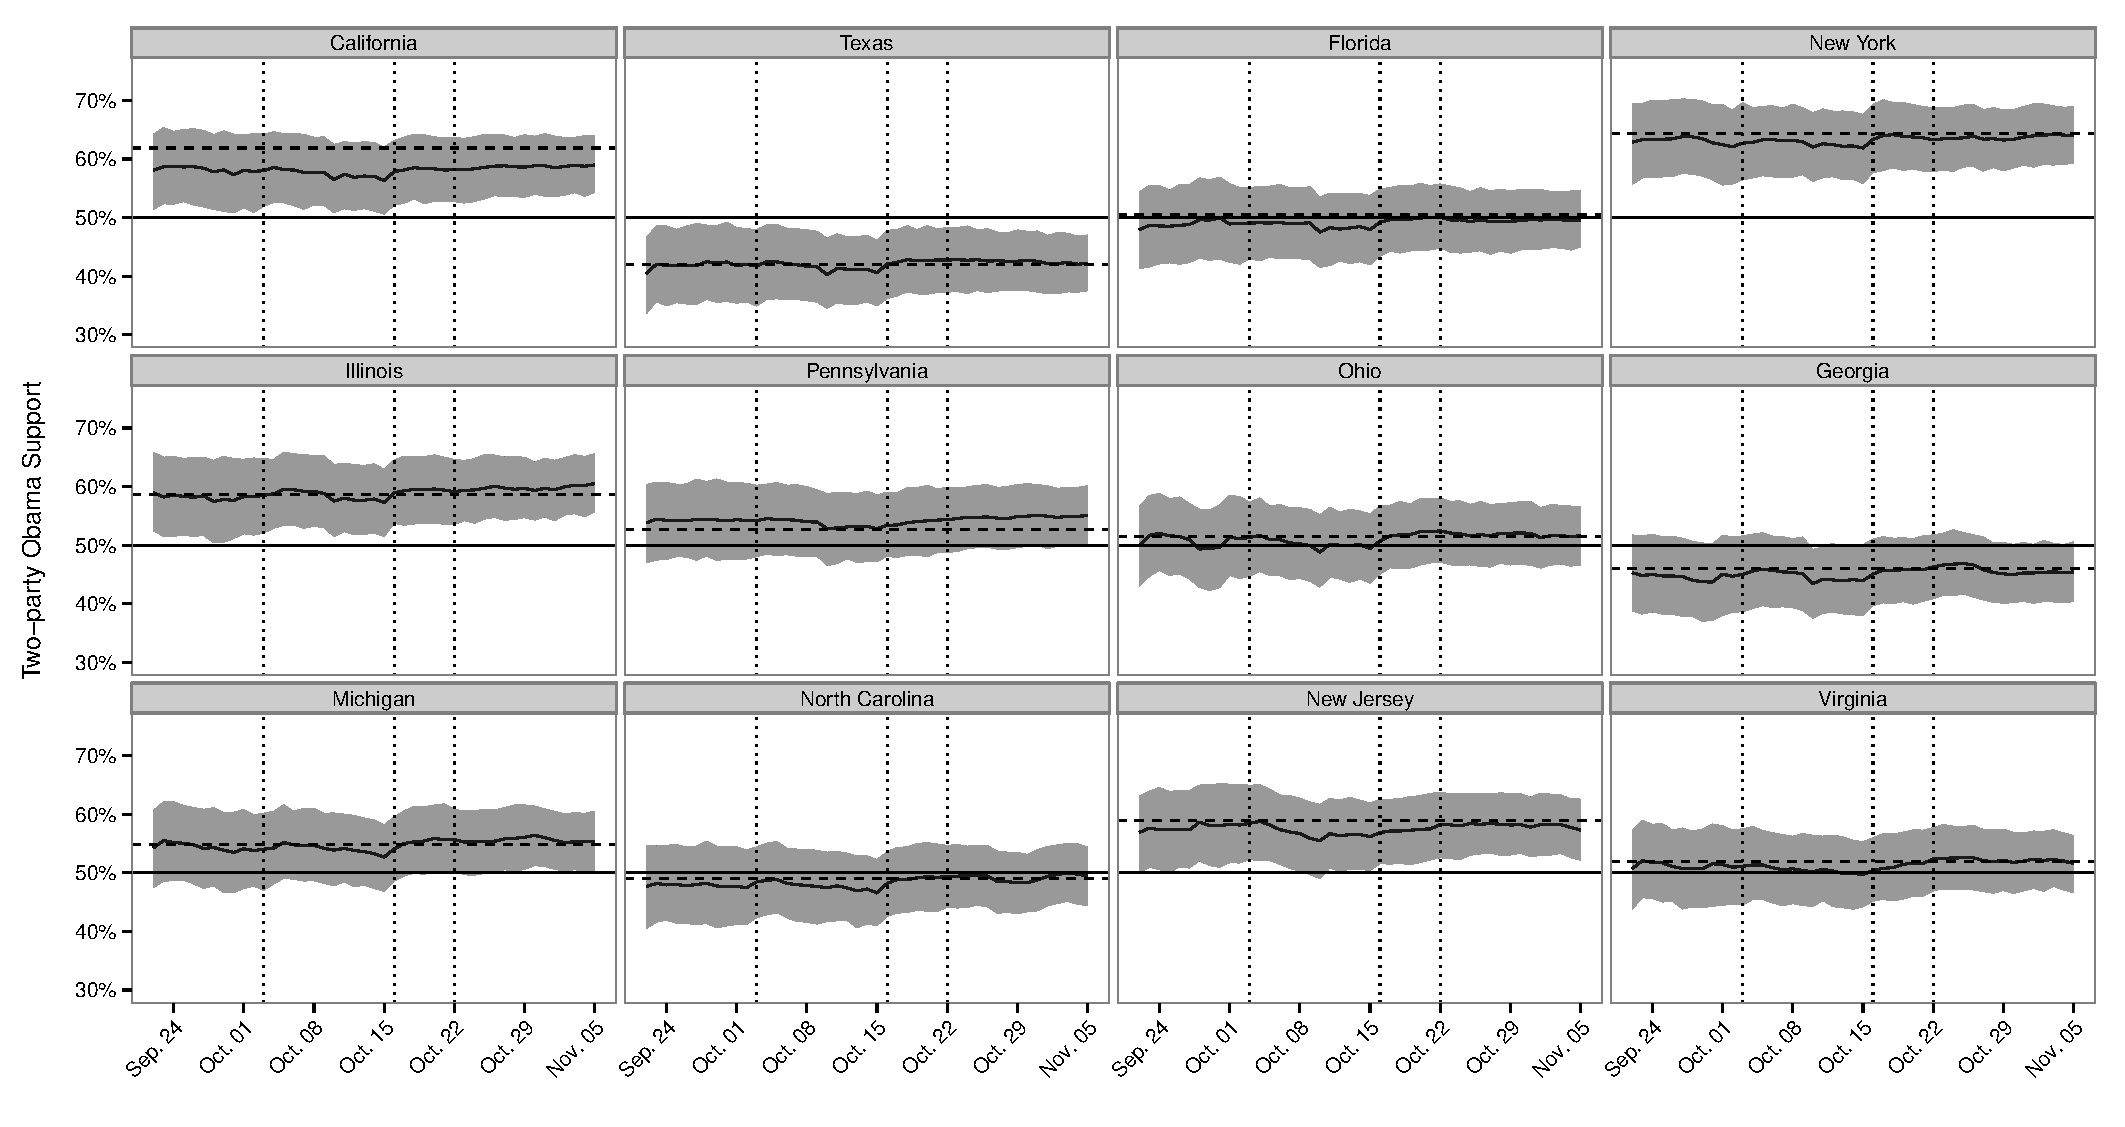
\includegraphics[width=\textwidth]{projected_voteshare_state}
  \caption{Projected Obama share of the two-party vote on election day
    for each of the 12 states
    with the most electoral votes, and associated 95\% confidence
    bands. Compared to the MRP-adjusted voter intent in Figure
    \ref{fig:state_snap}, the projected two-party Obama support is more stable, and the North Carolina race switches direction after applying the
    calibration model. Additionally, the confidence bands become much wider and
    give more reasonable state-by-state probabilities of Obama victories.}
  \label{fig:proj_state}
\end{figure}

\begin{figure}
  \centering
  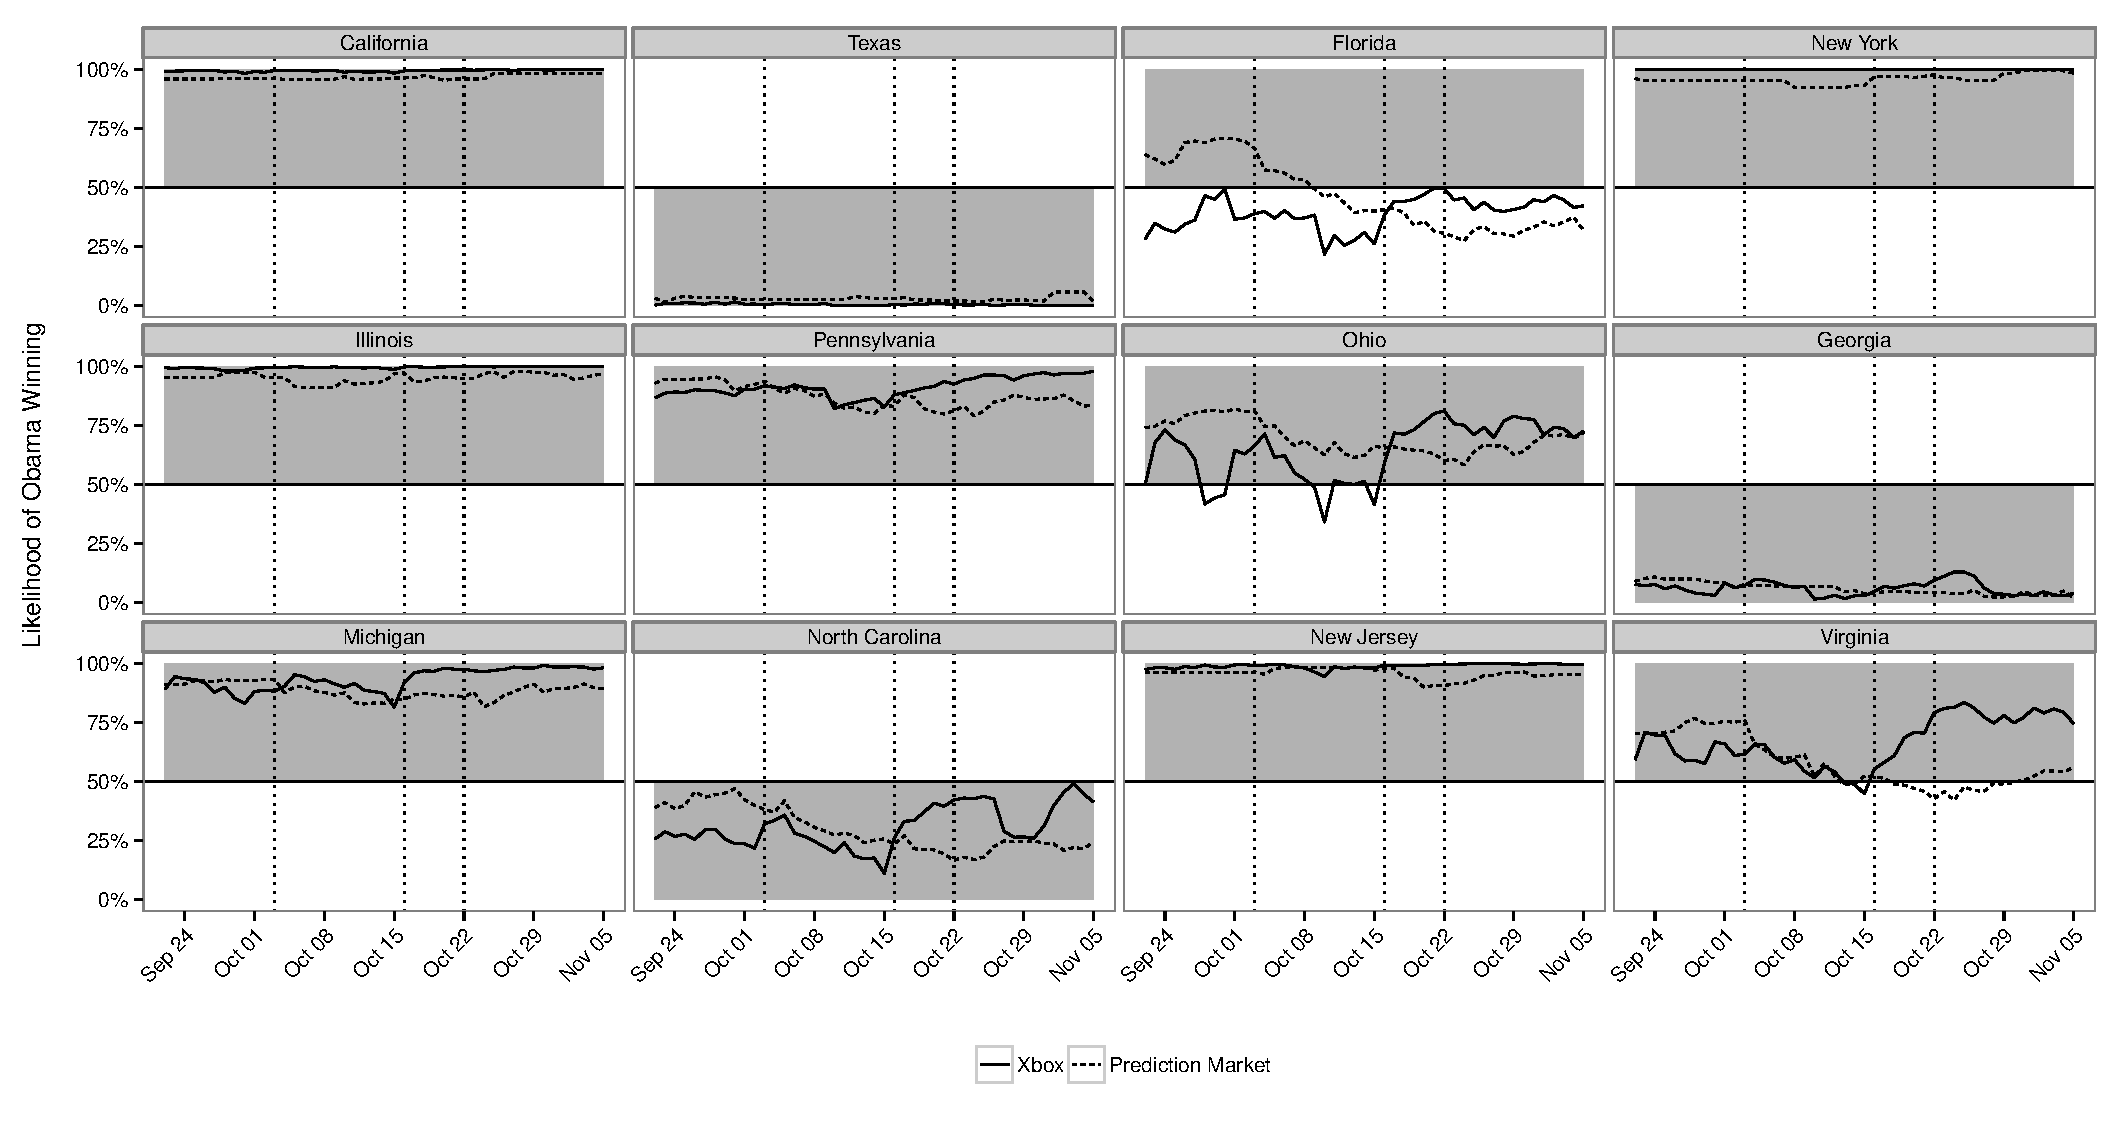
\includegraphics[width=\textwidth]{pred_market_xbox_comp}
  \caption{Comparison between the probability of Obama winning the 12 largest
    Electoral College races based on Xbox data and on prediction market
    data. The prediction market data are the average of the raw Betfair and Intrade
    prices from winner-take-all markets. The three vertical lines represent the
    dates of three presidential debates. The shaded halves indicate the direction
    that race went.}
  \label{fig:pm_comp}
\end{figure}

\begin{figure}
  \centering
  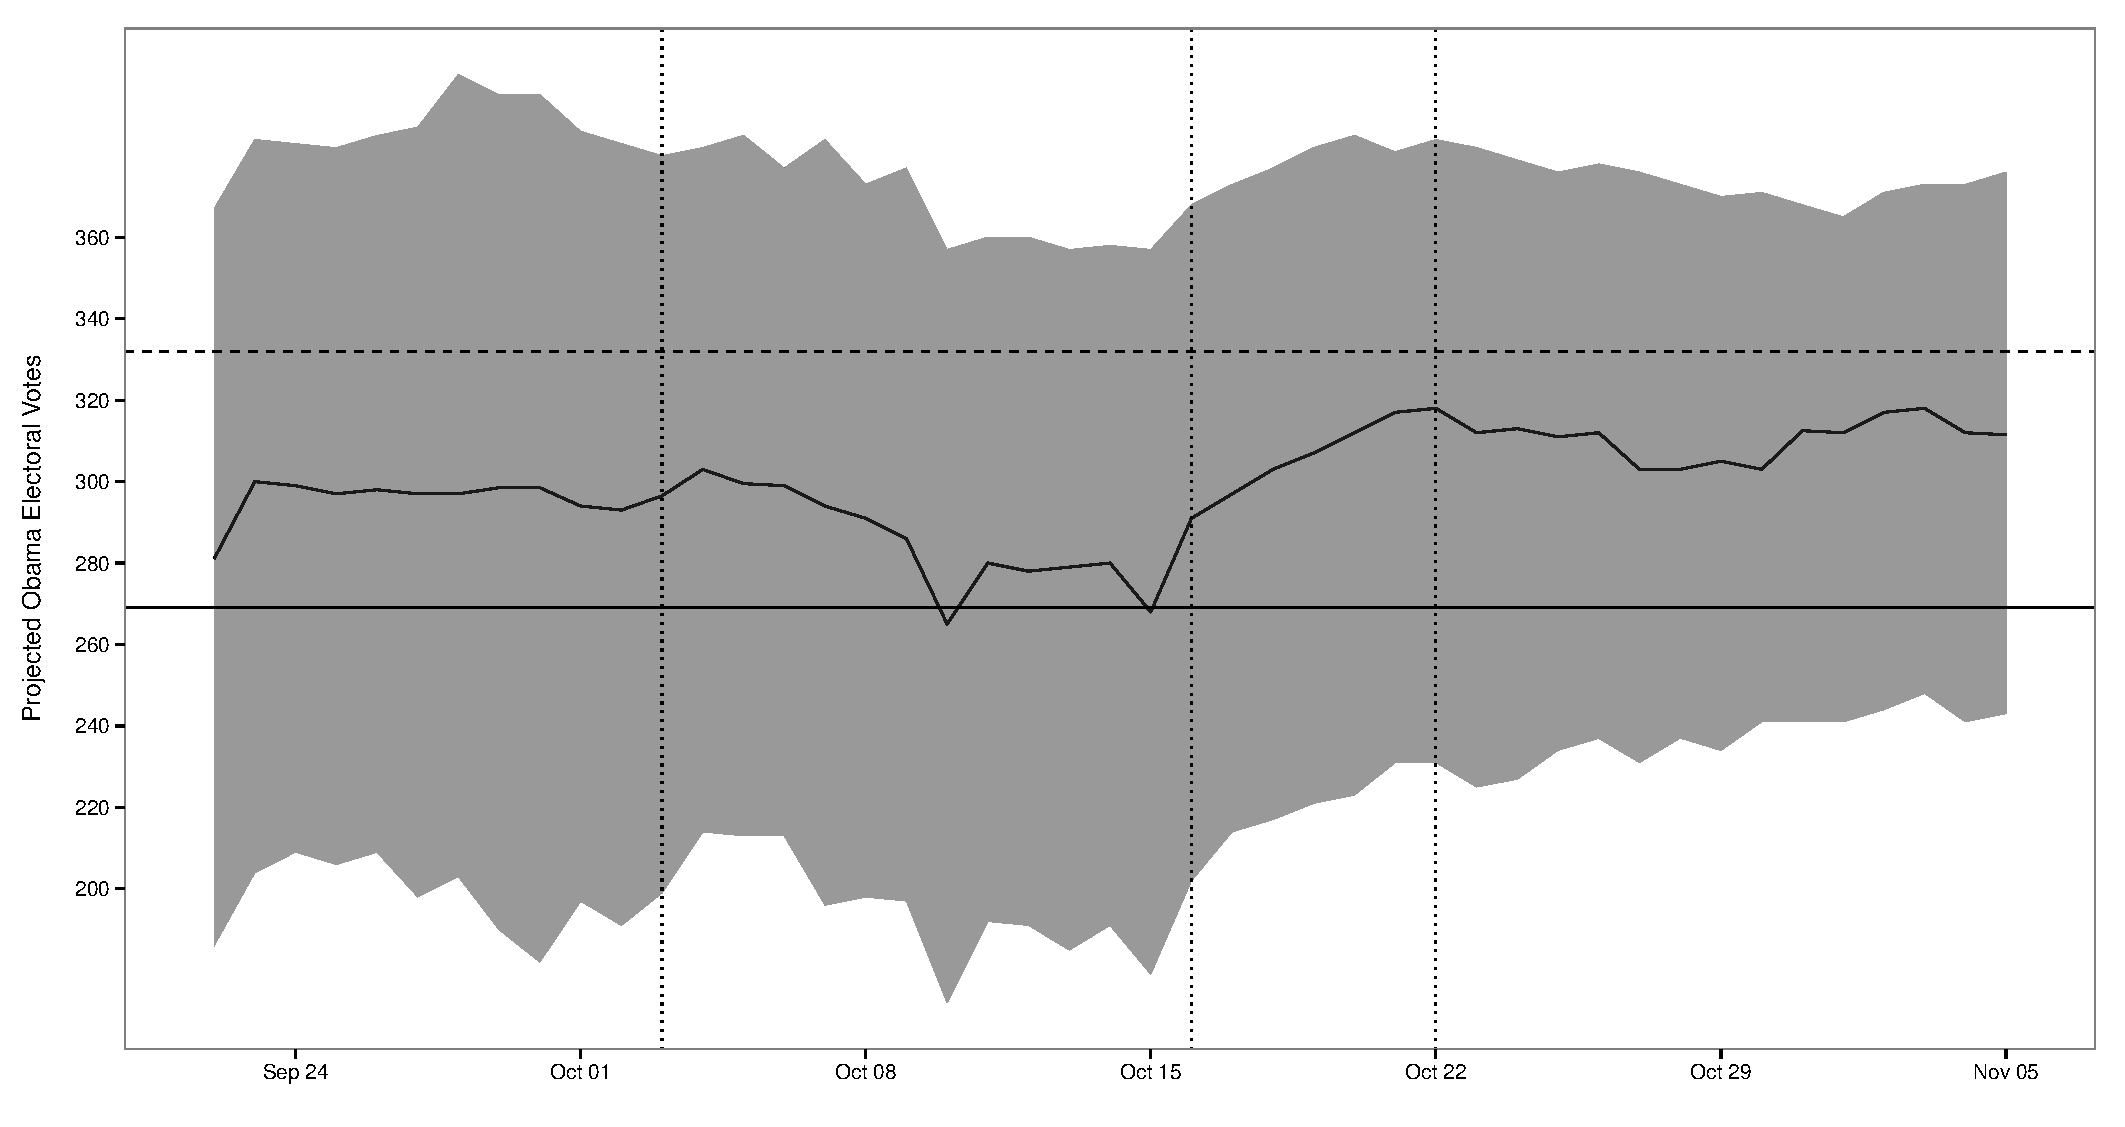
\includegraphics[width=\textwidth]{electoral_vote_dist_over_time}
  \caption{Daily projections of Obama electoral votes in the 45-day period
    leading up to the 2012 election and associated 95\% confidence bands. The
    solid line represents the median of the daily distribution. The horizontal
    dashed line represents the actual electoral votes, 332, that Obama captured
    in 2012 election. Three vertical dotted lines indicate the dates of three
    presidential debates.}
  \label{fig:ev_daily}
\end{figure}

\begin{figure}
  \centering
  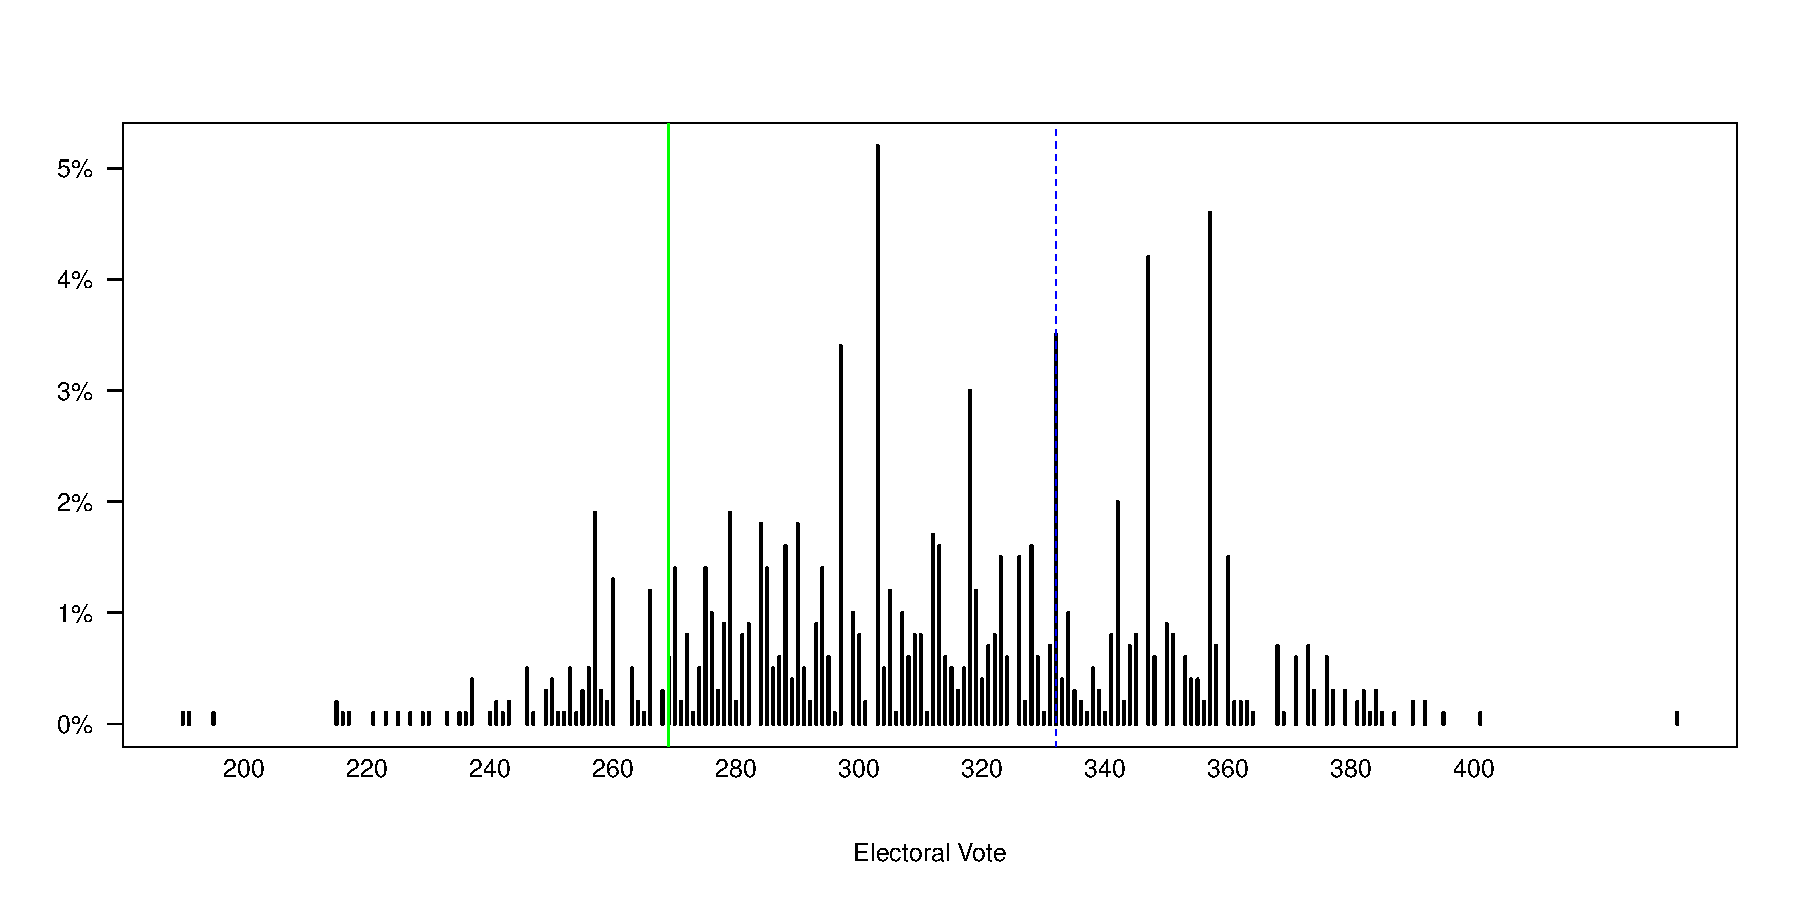
\includegraphics[width=\textwidth]{last_day_electoral_vote_dist}
  \caption{Projected distribution of electoral votes for Obama one day before the election. The green vertical dotted line represents 269, the minimum number of electoral votes that Obama needs for a tie. The blue vertical dashed line gives 332, the actual number of electoral votes captured by Obama. The estimated likelihood of Obama winning the electoral vote is 88\%.}
  \label{fig:ev_lastday}
\end{figure}

With the full state-level outcome distribution, we can also estimate the distribution of Electoral College votes.
Figure~\ref{fig:ev_daily} plots the median projected electoral votes for Obama over the last 45-days of the election,
together with the 95\% confidence band.
%Since we have the joint distribution of state level vote shares, the daily
%distribution of the electoral votes that Obama can capture on the election day is
%also generated, which is illustrated in Figure \ref{fig:ev_daily}.
In particular, on the day before the election, our model estimates Obama had an 88\% chance
of victory, in line with estimates based on traditional polling data. For example, Simon Jackman predicted Obama had a 91\% chance of victory, using a method built from \citet{jackman2005pooling}.
%we inspect the last day projection of Obama's electoral votes (shown in Figure
Zooming in on the day before the election, Figure~\ref{fig:ev_lastday} shows the
full predicted distribution of electoral votes for Obama.  Compared to the
actual 332 votes that Obama captured, we estimate a median of 312 votes, with the
most likely outcome being 303. Though this distribution of Electoral College
outcomes seems reasonable, it does appear to have higher variance than one might
expect. In particular, the extreme outcomes seem to have unrealistically high
likelihood of occurring, which is likely a byproduct of our calibration model
not fully capturing the state-level correlation structure.  Nonetheless, given
that our forecasts are based on a highly biased convenience sample of
respondents, the model predictions are remarkably good.

%It gives Obama winning the Electoral College a probability
%of 88\%, which largely agrees with the predictions made by poll analysts who
%aggregate standard polling results.


\section{Conclusion}
Forecasts not only need to be accurate, but also relevant, timely, and cost-effective. 
In this paper, we construct election forecasts satisfying all of these requirements using 
%demonstrate that such indicators of candidate support and forecasts of election outcomes can be created with those attributes with 
extremely non-representative data.
Though our data were collected on a proprietary polling platform, in principle one can aggregate such non-representative samples
at a fraction of the cost of conventional survey designs.
Moreover, the data produce forecasts that are both relevant and timely, as they can be updated faster and more regularly than standard election polls.
%the data is extremely cost-effective
%compared with the standard representative data;
%in many cases the data collection could be as low as 1\% of the cost. Further, we show that the same relevant outcomes can be generated and they are updated more regularly than standard polls.
Thus, the key question---and one of the main contributions of this paper---is to assess the extent to which one can generate accurate predictions from non-representative samples.
%is whether or not they are accurate.
Since there is limited ground truth for election forecasts, definitely establishing the accuracy of our predictions is difficult.
Nevertheless, we show that the MRP-adjusted and calibrated Xbox estimates are both intuitively reasonably, and are also quite similar to those generated by more traditional means.
%transformed non-representative data
% produces results similar to the more costly representative data and, knowing the outcomes, are extremely reasonable.


%The impact of the methods described in this paper will not be increased data on the presidential elections,
The greatest impact of non-representative polling will likely not be for presidential elections,
but rather for smaller, local elections and specialized survey settings, where it is impractical to deploy traditional methods
due to cost and time constraints.
%too costly to investigate with traditional polling or the research could benefit from the speed that samples of convenience supply.
For example, non-representative polls could be used in Congressional elections, where there are currently only sparse polling data.
%Due in part to cost, the General Social Survey is now conducted every other year, rather than yearly.
Non-representative polls could also supplement traditional surveys (e.g., the General Social Survey) by offering preliminary
results at shorter intervals.
%And, while traditional methods provide solid benchmarks,
%several key social science
%surveys have either scaled back their frequency or collapsed under their cost in the last few years (e.g., the General Social Survey, which is .
%Our methods can help supplement this data in the intervals.
Finally, when there is a need to identify and track pivotal events that affect public opinion, non-representative polling offers the possibility of
%gathering that data on a rolling basis and at a reasonable cost.
cost-effective continuous data collection.
Standard representative polling will certainly continue to be an invaluable tool for the foreseeable future. However,
75 years after the \textsl{Literary Digest} failure,
non-representative polling (followed by appropriate post-data adjustment) is due for further exploration, for
election forecasting and in social research more generally.
%---with proper statistical transformations---can provide similarly accurate answers to the same relevant questions, at a fraction of the cost and in a more timely manner, surely they are worth revisiting over

%% The Appendices part is started with the command \appendix;
%% appendix sections are then done as normal sections
%% \appendix

%% \section{}
%% \label{}

%% References
%%
%% Following citation commands can be used in the body text:
%%
%%  \cite{tkey}  ==>>  Jones et al. (1990)
%%  \citep{key}  ==>>  (Jones et al., 1990)
%%
%% Multiple citations as normal:
%% \citep{key1,key2}         ==>> (Jones et al., 1990; Smith, 1989)
%%                            or  (Jones et al., 1990, 1991)
%%                            or  (Jones et al., 1990a,b)
%% \cite{key} is the equivalent of \citet{key} in author-year mode
%%
%% Full author lists may be forced with \citet* or \citep*, e.g.
%%   \citep*{key}            ==>> (Jones, Baker, and Williams, 1990)
%%
%% Optional notes as:
%%   \citep[chap. 2]{key}    ==>> (Jones et al., 1990, chap. 2)
%%   \citep[e.g.,][]{key}    ==>> (e.g., Jones et al., 1990)
%%   \citep[see][pg. 34]{key}==>> (see Jones et al., 1990, pg. 34)
%%  (Note: in standard LaTeX, only one note is allowed, after the ref.
%%   Here, one note is like the standard, two make pre- and post-notes.)
%%
%%   \citealt{key}          ==>> Jones et al. 1990
%%   \citealt*{key}         ==>> Jones, Baker, and Williams 1990
%%   \citealp{key}          ==>> Jones et al., 1990
%%   \citealp*{key}         ==>> Jones, Baker, and Williams, 1990
%%
%% Additional citation possibilities
%%   \citeauthor{key}       ==>> Jones et al.
%%   \citeauthor*{key}      ==>> Jones, Baker, and Williams
%%   \citeyear{key}         ==>> 1990
%%   \citeyearpar{key}      ==>> (1990)
%%   \citetext{priv. comm.} ==>> (priv. comm.)
%%   \citenum{key}          ==>> 11 [non-superscripted]
%% Note: full author lists depends on whether the bib style supports them;
%%       if not, the abbreviated list is printed even when full requested.
%%
%% For names like della Robbia at the start of a sentence, use
%%   \Citet{dRob98}         ==>> Della Robbia (1998)
%%   \Citep{dRob98}         ==>> (Della Robbia, 1998)
%%   \Citeauthor{dRob98}    ==>> Della Robbia


%% References with bibTeX database:

\bibliographystyle{elsarticle-harv}
\bibliography{xbox_forecast}

%% Authors are advised to submit their bibtex database files. They are
%% requested to list a bibtex style file in the manuscript if they do
%% not want to use elsarticle-harv.bst.

%% References without bibTeX database:

% \begin{thebibliography}{00}

%% \bibitem must have one of the following forms:
%%   \bibitem[Jones et al.(1990)]{key}...
%%   \bibitem[Jones et al.(1990)Jones, Baker, and Williams]{key}...
%%   \bibitem[Jones et al., 1990]{key}...
%%   \bibitem[\protect\citeauthoryear{Jones, Baker, and Williams}{Jones
%%       et al.}{1990}]{key}...
%%   \bibitem[\protect\citeauthoryear{Jones et al.}{1990}]{key}...
%%   \bibitem[\protect\astroncite{Jones et al.}{1990}]{key}...
%%   \bibitem[\protect\citename{Jones et al., }1990]{key}...
%%   \harvarditem[Jones et al.]{Jones, Baker, and Williams}{1990}{key}...
%%

% \bibitem[ ()]{}

% \end{thebibliography}

\end{document}

%%
%% End of file `elsarticle-template-harv.tex'.
